\p
طبق شرایط مسئله صفحه را به دل‌خواه، به موزاییک‌های 
$3\times1$ 
تقسیم می‌کنیم. بدیهی است که یک خانه اضافه می‌آید.
	\p
\begin{center}
    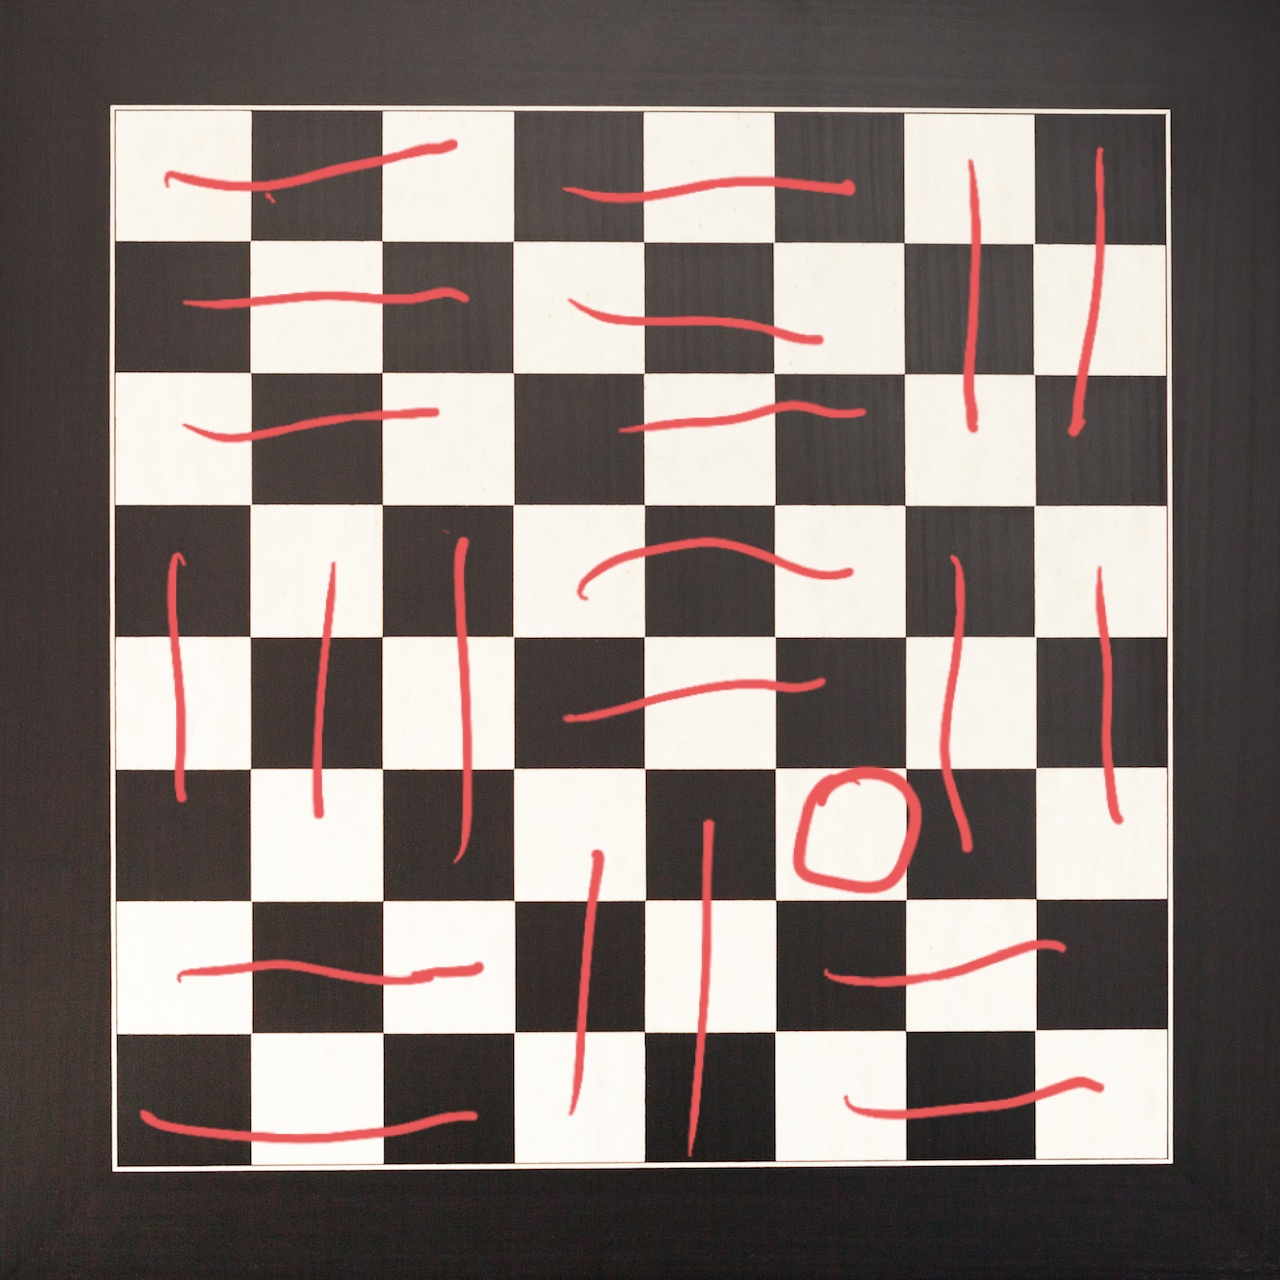
\includegraphics[height=5cm]{Q3Pic.jpg}
\end{center}
	\p
 در حالتی که آن خانه بنفش باشد، در
$21$ 
موزاییک ایجاد شده حداقل
$43$
خانه رنگ شده وجود دارد، پس بر اساس اصل لانه کبوتری حداقل 
$1$
موزاییک وجود دارد که هر 
$3$ 
خانه‌اش رنگ شده باشد:
\[[\frac {43} {21}]+1=3\]  
در حالتی که خانه اضافه بنفش نباشد نیز:
\[[\frac {44} {21}]+1=3\]  
بنابراین 
$3$
 خانه متوالی در یک سطر یا ستون وجود دارند که هر سه به رنگ بنفش باشند.